\begin{frame}[fragile]
  \frametitle{M\'odulos y paquetes}

  \framesubtitle{Paquetes}

  Si los m\'odulos sirven para organizar el c\'odigo, los paquetes sirven para organizar los m\'odulos. Los paquetes son tipos especiales de m\'odulos (ambos son de tipo module) que permiten agrupar m\'odulos relacionados.Se representan mediante directorios.

  \begin{figure}
    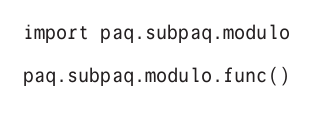
\includegraphics[width=0.6\textwidth]{Imagenes/Paquetes.jpg}
    \caption{\label{fig:Ejemplo12}Ejemplo de paquetes en Python.}
  \end{figure}

 

\end{frame}
